\documentclass[a4paper,11pt]{article}

\usepackage[top=1in, bottom=1in, left=1in, right=1in]{geometry}
\usepackage{hyperref}
\usepackage{amsmath, amssymb}
\usepackage{enumitem}
\usepackage{graphicx}
\usepackage[labelformat=empty]{caption}
\usepackage{tcolorbox}
\tcbuselibrary{breakable}
\usepackage{multicol}
\usepackage{tabularx}
\usepackage{ltablex}
\usepackage{centernot}

\title{Calculus Notes}
\author{Abror Maksudov}
\date{Last Updated: \today}

\everymath{\displaystyle}

\begin{document}

\maketitle
\tableofcontents

\section{Limits}


% PRECISE DEFINITION OF A LIMIT


\subsection{Precise Definition of a Limit}

\begin{tcolorbox}
    \textbf{Standard Limit:}  
    \[
    \lim_{x \to a} f(x) = L \quad \text{if} \quad \forall \varepsilon > 0, \, \exists \delta > 0 \text{ such that } 0 < |x - a| < \delta \Rightarrow |f(x) - L| < \varepsilon.
    \]
\end{tcolorbox}


% PRECISE DEFINITION OF ONE-SIDED LIMIT

\subsection{Precise Definition of One-Sided Limit}

\begin{tcolorbox}
    \textbf{Right-Hand Limit:}  
    \[
    \lim_{x \to a^+} f(x) = L \quad \text{if} \quad \forall \varepsilon > 0, \, \exists \delta > 0 \text{ such that } 0 < x - a < \delta \Rightarrow |f(x) - L| < \varepsilon.
    \]
    \textbf{Left-Hand Limit:}  
    \[
    \lim_{x \to a^-} f(x) = L \quad \text{if} \quad \forall \varepsilon > 0, \, \exists \delta > 0 \text{ such that } 0 < a - x < \delta \Rightarrow |f(x) - L| < \varepsilon.
    \]
\end{tcolorbox}


% PRECISE DEFINITION OF INFINITE LIMIT


\subsection{Precise Definition of Infinite Limit}

\begin{tcolorbox}
    \textbf{Infinite Limit:}  
    \[
    \lim_{x \to a} f(x) = \infty \quad \text{if} \quad \forall M > 0, \, \exists \delta > 0 \text{ such that } 0 < |x - a| < \delta \Rightarrow f(x) > M.
    \]
    \[
    \lim_{x \to a} f(x) = -\infty \quad \text{if} \quad \forall M > 0, \, \exists \delta > 0 \text{ such that } 0 < |x - a| < \delta \Rightarrow f(x) < -M.
    \]
\end{tcolorbox}


% PRECISE DEFINITION OF LIMIT AT INFINITY


\subsection{Precise Definition of a Limit at Infinity}

\begin{tcolorbox}
    \textbf{Limit at Infinity:}
    \[
    \lim_{x \to \infty} f(x) = L \quad \text{if} \quad \forall \varepsilon > 0, \, \exists M > 0 \text{ such that } x > M \Rightarrow |f(x) - L| < \varepsilon.
    \]
    \[
    \lim_{x \to -\infty} f(x) = L \quad \text{if} \quad \forall \varepsilon > 0, \, \exists M > 0 \text{ such that } x < -M \Rightarrow |f(x) - L| < \varepsilon.
    \]
\end{tcolorbox}


% PRECISE DEFINITION OF INFINITE LIMIT AT INFINITY


\subsection{Precise Definition of Infinite Limit at Infinity}

\begin{tcolorbox}
    \textbf{Infinite Limit at Infinity:}  
    \[
    \lim_{x \to \infty} f(x) = \infty \quad \text{if} \quad \forall M > 0, \, \exists N > 0 \text{ such that } x > N \Rightarrow f(x) > M.
    \]
    \[
    \lim_{x \to \infty} f(x) = -\infty \quad \text{if} \quad \forall M > 0, \, \exists N > 0 \text{ such that } x > N \Rightarrow f(x) < -M.
    \]
    \[
    \lim_{x \to -\infty} f(x) = \infty \quad \text{if} \quad \forall M > 0, \, \exists N > 0 \text{ such that } x < -N \Rightarrow f(x) > M.
    \]
    \[
    \lim_{x \to -\infty} f(x) = -\infty \quad \text{if} \quad \forall M > 0, \, \exists N > 0 \text{ such that } x < -N \Rightarrow f(x) < -M.
    \]
\end{tcolorbox}


% LIMIT LAWS


\subsection{Limit Laws}

\begin{tcolorbox}
    Suppose that $c$ is a constant and the limits $ \lim_{x \to a} f(x)$ and $ \lim_{x \to a} g(x)$ exist. Then
    \begin{enumerate}
        \item $\lim_{x \to a} c = c$
        \item $\lim_{x \to a} x = a$
        \item $\lim_{x \to a} [f(x) \pm g(x)] = \lim_{x \to a} f(x) \pm \lim_{x \to a} g(x)$
        \item $\lim_{x \to a} [c f(x)] = c \lim_{x \to a} f(x)$
        \item $\lim_{x \to a} [f(x) g(x)] = \lim_{x \to a} f(x) \cdot \lim_{x \to a} g(x)$
        \item $\lim_{x \to a} \frac{f(x)}{g(x)} = \frac{\displaystyle \lim_{x \to a} f(x)}{\lim_{x \to a} g(x)},\ \text{if } \lim_{x \to a} g(x) \neq 0$
        \item $\lim_{x \to a} [f(x)]^n = [\lim_{x \to a} f(x)]^n$
        \item $\lim_{x \to a} \sqrt[n]{f(x)} = \sqrt[n]{\lim_{x \to a} f(x)}$
    \end{enumerate}
\end{tcolorbox}


% RELATIONSHIP BETWEEN THE LIMIT AND ONE-SIDED LIMITS


\subsection{Relationship between the Limit and One-Sided Limits}

\begin{tcolorbox}
    \[
    \lim_{x \to a} f(x) = L \iff \lim_{x \to a^+} f(x) = \lim_{x \to a^-} f(x) = L.
    \]
    \[
    \lim_{x \to a^+} f(x) \neq \lim_{x \to a^-} f(x) \implies \lim_{x \to a} f(x) \text{ does not exist}.
    \]
\end{tcolorbox}


% COMPARISON THEOREM


\subsection{Comparison Theorem}

\begin{tcolorbox}
    If  $f(x) \leq g(x)$ when $x$ is near $a$, and $\lim_{x \to a} f(x)$ and $\lim_{x \to a} g(x)$ exist, then 
    \[
    \lim_{x \to a} f(x) \leq \lim_{x \to a} g(x).
    \]
\end{tcolorbox}


% SQUEEZE THEOREM


\subsection{Squeeze Theorem}

\begin{tcolorbox}
    If $f(x) \leq g(x) \leq h(x)$ when $x$ is near $a$, then
    \[ 
    \lim\limits_{x \to a} f(x) = \lim\limits_{x \to a} h(x) = L \implies \lim\limits_{x \to a} g(x) = L.
    \]
\end{tcolorbox}


% CONTINUITY


\subsection{Continuity}

\begin{tcolorbox}
    A function $f(x)$ is \textbf{continuous at} $x = a$ if and only if it satisfies \textbf{all} the following:
    \[
    \begin{aligned}
        &\text{(1)} \quad f(a) \text{ exists} \\  
        &\text{(2)} \quad \lim\limits_{x \to a} f(x) \text{ exists} \\  
        &\text{(3)} \quad \lim\limits_{x \to a} f(x) = f(a)  
    \end{aligned}
    \]
    Otherwise, $f(x)$ is discontinuous at $x = a$.
\end{tcolorbox}


% PROPERTIES OF CONTINUOUS FUNCTIONS


\subsection{Properties of Continuous Functions}


\begin{tcolorbox}
    If $f(x)$ and $g(x)$ are continuous at $x = a$ and $c$ is a constant, then the following functions are also continuous at $x = a$:  
    \begin{enumerate}
        \begin{multicols}{3}
            \item $f + g$
            \item $f - g$
            \item $cf$
        \end{multicols}
        \begin{multicols}{3}
            \item $fg$
            \item $\frac{f}{g} \quad$ if $g(a) \neq 0$
        \end{multicols}
    \end{enumerate}
\end{tcolorbox}



% TYPES OF DISCONTINUITY


\subsection{Types of Discontinuity}

\begin{figure}[htbp]
    \centering
    \includegraphics[width=\textwidth]{4-types-of-discontinuity.png} 
    \caption{Source: calcworkshop.com}
    \label{fig:discontinuity}
\end{figure}


% LIMITS OF CONTINUOUS FUNCTIONS


\subsection{Limits of Continuous Functions}

\begin{tcolorbox}
    If $f(x)$ is continuous at $b$ and $\lim_{x \to a} g(x) = b$,  then
    \[
    \lim_{x \to a} f(g(x)) = f( \lim_{x \to a} g(x) ) = f(b).
    \]
    \tcblower
    If $g$ is continuous at $a$ and $a$ is continuous at $g(a)$, then the composite $f \circ g$ is continuous at $a$.
\end{tcolorbox}


% INTERMEDIATE VALUE THEOREM


\subsection{Intermediate Value Theorem}

\begin{tcolorbox}
    If $f$ is continuous on a closed interval $[a, b]$, then for any $N$ between $f(a)$ and $f(b)$,  
    \[
    \exists c \in [a,b] \text{ such that } f(c) = N
    \]
\end{tcolorbox}


% ASYMPTOTES


\subsection{Asymptotes}

\begin{tcolorbox}[breakable]
    \textbf{Vertical Asymptote:} 
    $x = a$ is a vertical asymptote if  
    \[
    \lim_{x \to a^{\pm}} f(x) = \pm \infty.
    \]
    
    \textbf{Horizontal Asymptote:}
    $y = L$ is a horizontal asymptote if  
    \[
    \lim_{x \to \pm \infty} f(x) = L.
    \]
    For $f(x) = \frac{P(x)}{Q(x)}$, compare degrees of $P$ and $Q$:  
    \[
    \begin{aligned}
        &\deg P < \deg Q \quad \implies \quad y = 0. \\  
        &\deg P = \deg Q \quad \implies \quad y = \frac{\text{leading coef. of } P}{\text{leading coef. of } Q}. \\  
        &\deg P > \deg Q \quad \implies \quad \text{no horizontal asymptote}.
    \end{aligned}
    \]

    \textbf{Oblique Asymptote:}
    $y = mx + b$ is an oblique asymptote if  
    \[
    \lim_{x \to \pm \infty} [f(x) - (mx + b)] = 0.
    \]
    For a rational function $f(x) = \frac{P(x)}{Q(x)}$, if $\deg P = \deg Q + 1$, then $f(x)$ has an oblique asymptote.  
    Find it by polynomial long division:  
    \[
    f(x) = D(x) + \frac{R(x)}{Q(x)}, \quad \text{as } x \to \pm \infty, \quad f(x) \approx D(x).
    \]
    
    \textbf{Curvilinear Asymptote:}
    $y = g(x)$ is a curvilinear asymptote if
    \[
    \lim_{x \to \pm \infty} [f(x) - g(x)] = 0,
    \]
    where $g(x)$ is any non-linear function.
\end{tcolorbox}


% COMMON LIMITS


\subsection{Common Limits}

\begin{tcolorbox}
    Assume $a > 0$ in the following.
    \begin{multicols}{2}
        \begin{enumerate}
            \item $\lim_{x \to 0} \frac{\sin ax}{bx} = \frac{a}{b}$
            \item $\lim_{x \to 0} \frac{1 - \cos x}{x} = 0$
            \item $\lim_{x \to 0} \frac{1 - \cos x}{x^2} = \frac{1}{2}$
            \item $\lim_{x \to 0} \frac{e^{ax} - 1}{x} = a$
            \item $\lim_{x \to 0} \frac{a^x - 1}{x} = \ln a$
            \item $\lim_{x \to \infty} \left(1 + \frac{k}{x}\right)^{mx} = e^{mk}$
            \item $\lim_{x \to 0} \frac{\ln(1 + x)}{x} = 1$
            \item $\lim_{x \to 0} \frac{\log_a(1 + x)}{x} = \log_a e$
            \item $\lim_{x \to 0^+} x^x = 1$
            \item $\lim_{x \to \infty} \sqrt[x]{x} = \lim_{x \to \infty} x^{\frac{1}{x}} = 1$
            \item $\lim_{x \to 0^+} x^a \ln x = 0$
            \item $\lim_{x \to \infty} x^{-a} \ln x = 0$
            \item $\lim_{n \to \infty} \frac{x^n}{n!} = 0 \lim\limits$
            \item \( \lim_{n \to \infty} \frac{n^n}{n!} = \infty \)
        \end{enumerate}
    \end{multicols}
\end{tcolorbox}


% --------------------------------------------------


\section{Derivatives}


% DERIVATIVE AT A POINT


\subsection{Derivative at a Point}

\begin{tcolorbox}
    The \textbf{derivative} of \( f(x) \) at \( x = a \) is the \textbf{instantaneous rate of change} at that point:
    \[
    f'(a) = \left. \frac{df}{dx} \right|_{x=a} =\lim\limits_{h \to 0} \frac{f(a + h) - f(a)}{h} = \lim\limits_{x \to a} \frac{f(x) - f(a)}{x - a}.
    \]
\end{tcolorbox}


% DERIVATIVE AT A POINT


\subsection{Derivative as a Function}

\begin{tcolorbox}
    The derivative of a function \( f(x) \) at a point \( x \) is defined as the limit
    \[
    f'(x) = \lim_{\Delta x \to 0} \frac{f(x + \Delta x) - f(x)}{\Delta x}.
    \]
\end{tcolorbox}


% DIFFERENTIABILITY


\subsection{Differentiability}

\begin{tcolorbox}
    A function \( f(x) \) is \textbf{differentiable} at \( x = a \) if its derivative \( f'(x) \) exists. That is:  
    \[
    f(x) \text{ is differentiable at } x = a \iff \text{ The limit } \lim\limits_{h \to 0} \frac{f(a+h) - f(a)}{h} \text{ exists.}
    \]
\end{tcolorbox}


% DIFFERENTIABILITY IMPLIES CONTINUITY


\subsection{Differentiability Implies Continuity}

\begin{tcolorbox}
    If \( f(x) \) is differentiable at \( x = a \), then it is continuous at \( x = a: \)
    \[
    f \text{ differentiable at } a \implies f \text{ continuous at } a.
    \]
    However, the converse is false:
    \[
    f \text{ continuous at } a \centernot\implies f \text{ differentiable at } a.
    \]
\end{tcolorbox}


% PROPERTIES OF DERIVATIVES


\subsection{Properties of Derivatives}

\begin{tcolorbox}
    Let $f(x)$ and $g(x)$ be differentiable functions. Then the following rules hold:
    \[
    \begin{aligned}
        &\text{(1)} \quad \frac{d}{dx}(c) = 0. \\[8pt]  
        &\text{(2)} \quad \frac{d}{dx}(x^n) = nx^{n-1}. \\[8pt]
        &\text{(3)} \quad \frac{d}{dx}[cf(x)] = c[\frac{d}{dx}f(x)]. \\[8pt]
        &\text{(4)} \quad \frac{d}{dx}[f(x) \pm g(x)] = \frac{d}{dx}f(x) \pm \frac{d}{dx}g(x). \\[8pt]
        &\text{(5)} \quad \frac{d}{dx}[f(x)g(x)] = f'(x)g(x) + f(x)g'(x). \\[8pt]
        &\text{(6)} \quad \frac{d}{dx}[\frac{f(x)}{g(x)}] = \frac{f'(x)g(x) - f(x)g'(x)}{g(x)^2}. \\[8pt]
        &\text{(7)} \quad \frac{d}{dx}[f(g(x))] = f'(g(x))g'(x). \\[8pt]
    \end{aligned}
    \]
\end{tcolorbox}


% TABLE OF DERIVATIVES


\subsection{Table of Derivatives}

\begin{tcolorbox}
    \begin{tabularx}{\textwidth}{X|X|X}
         $(\sin x)' = \cos x$ & 
         $(\arcsin x)' = \frac{1}{\sqrt{1-x^2}}$ & 
         $(e^x)' = e^x$ \\[10pt]
         
         $(\cos x)' = -\sin x$ & 
         $(\arccos x)' = -\frac{1}{\sqrt{1-x^2}}$ & 
         $(a^x)' = a^x\ln{a}$ \\[10pt]
         
         $(\tan x)' = \sec^2 x$ & 
         $(\arctan x)' = \frac{1}{1+x^2}$ & 
         $(\log_a{x})' = \frac{1}{x\ln{a}}$ \\[10pt]
         
         $(\cot x)' = -\csc^2 x$ & 
         $(\arccot x)' = -\frac{1}{1+x^2}$ & 
         $(\ln{x})' = \frac{1}{x}$ \\[10pt]
         
         $(\sec x)' = \sec x \tan x $ & 
         $(\arcsec x)' = \frac{1}{x\sqrt{x^2-1}}$ & 
         $(\left| x \right|)' = \frac{x}{|x|}$ \\[10pt]
         
         $(\csc x)' = -\csc x \cot x $ & 
         $(\arccsc x)' = -\frac{1}{x\sqrt{x^2-1}}$ & 
         $(x^x)' = x^x(1+\ln{x})$ \\[10pt]
    \end{tabularx}
\end{tcolorbox}



% ABSOLUTE AND LOCAL EXTREMA


\subsection{Absolute and Local Extrema}

\begin{tcolorbox}
    Let $f$ be defined on a domain $D$, and let $c \in D$.
    \begin{itemize}
        \item \textbf{Absolute Maximum:} $f(c)$ is an absolute maximum if $f(c) \geq f(x),\ \forall x \in D.$
        \item \textbf{Absolute Minimum:} $f(c)$ is an absolute minimum if $f(c) \leq f(x),\ \forall x \in D.$
        \item \textbf{Local Maximum:} $f(c)$ is a local maximum if $\exists \delta > 0$ such that $f(c) \geq f(x),\\ \quad \forall x \in (c - \delta, c + \delta).$
        \item \textbf{Local Minimum:} $f(c)$ is a local minimum if $\exists \delta > 0$ such that $f(c) \leq f(x),\\ \quad \forall x \in (c - \delta, c + \delta).$
    \end{itemize}
\end{tcolorbox}


% EXTREME VALUE THEOREM


\subsection{Extreme Value Theorem}

\begin{tcolorbox}
    If $f$ is continuous on a closed interval $[a,b]$, then $f$ attains an absolute maximum and an absolute minimum on $[a,b]$:
    \[
    \exists c,d \in [a,b] \text{ such that } f(c) \leq f(x) \leq f(d),\quad \forall x \in [a,b].
    \]
\end{tcolorbox}


% CRITICAL AND STATIONARY POINTS


\subsection{Critical and Stationary Points}

\begin{tcolorbox}
    Let $f$ be defined on an interval $I$ and $c \in I.$
    \begin{itemize}
        \item \textbf{Critical Point:} $c$ is a critical point of $f$ if either
        \begin{enumerate}
            \item $f'(c) = 0$, or
            \item $f'(c)$ does not exist
        \end{enumerate}
        \item \textbf{Stationary Point:} $c$ is a stationary point of $f$ if $f'(c) = 0.$        
    \end{itemize}
    Note: \textit{Every stationary point is a critical point, but not conversely.}
\end{tcolorbox}


% ROLLE'S THEOREM


\subsection{Rolle's Theorem}

\begin{tcolorbox}
    Let $f$ satisfy all conditions:
    \begin{enumerate}
        \item $f$ is continuous on $[a,b]$.
        \item $f$ is differentiable on $(a,b)$.
        \item $f(a) = f(b)$.
    \end{enumerate}
    Then, there exists at least one $c \in (a,b)$ such that $f'(c) = 0$.
\end{tcolorbox}


% MEAN VALUE THEOREM


\subsection{Mean Value Theorem}

\begin{tcolorbox}
    Let $f$ satisfy all conditions:
    \begin{enumerate}
        \item $f$ is continuous on $[a,b]$.
        \item $f$ is differentiable on $(a,b)$.
    \end{enumerate}
    Then, there exists at least one $c \in (a,b)$ such that:
    \[
    f'(c) = \frac{f(b) - f(a)}{b-a}.
    \]
    Note: Rolle's Theorem is a special case of the Mean Value Theorem where $f(a) = f(b)$.
\end{tcolorbox}


% INCREASING/DECREASING TEST


\subsection{Increasing/Decreasing Test}

\begin{tcolorbox}
    Let $f$ be differentiable on an interval $I$. Then, for all $x \in I$:
    \begin{enumerate}
        \item If $f'(x) > 0$, then $f$ is strictly increasing on $I$.
        \item If $f'(x) < 0$, then $f$ is strictly decreasing on $I$.
        \item If $f'(x) = 0$, then $f$ is constant on $I$.
    \end{enumerate}
\end{tcolorbox}


% FIRST DERIVATIVE TEST


\subsection{First Derivative Test}

\begin{tcolorbox}
    Let $c$ be a critical point of a differentiable function $f(x)$, meaning $f'(c)=0$ or $f'(c)$ does not exist. Then:
    \begin{enumerate}
        \item If $f'(x)$ changes from positive to negative at $x=c$, then $f(c)$ is a \textbf{local maximum}.
        \item If $f'(x)$ changes from negative to positive at $x=c$, then $f(c)$ is a \textbf{local minimum}.
        \item If $f'(x)$ does not change sign at $x=c$, then $f(c)$ is \textbf{neither} a local maximum nor a local minimum.
    \end{enumerate}
\end{tcolorbox}


% CONCAVITY AND INFLECTION POINTS


\subsection{Concavity and Inflection Points}

\begin{tcolorbox}
    \[\text{Concave up} \iff \text{Curve \textbf{lies above} all of its \textbf{tangent lines}}.\]
    \[\text{Concave down} \iff \text{Curve \textbf{lies below} all of its \textbf{tangent lines}}.\]
    \[\text{Inflection point} \iff \text{Point where \textbf{concavity changes}}.\]
\end{tcolorbox}


% CONCAVITY TEST


\subsection{Concavity Test}

\begin{tcolorbox}
    Let $f(x)$ be twice differentiable on interval $I$. Then:
    \begin{itemize}
        \item If $f''(x) > 0, \quad \forall x \in I \implies f(x)$ is \textbf{concave up} on $I$.
        \item If $f''(x) < 0, \quad \forall x \in I \implies f(x)$ is \textbf{concave down} on $I$.
    \end{itemize}
\end{tcolorbox}


% SECOND DERIVATIVE TEST


\subsection{Second Derivative Test}

\begin{tcolorbox}
    Let $c$ be a critical point of $f$ where $f(c)=0$. If $f''(c)$ exists, then:
    \begin{enumerate}
        \item If $f''(c) > 0$, $f(x)$ is \textbf{concave up} at $c$, so $f(c)$ is a \textbf{local minimum}.
        \[ \text{Local Maximum at $c$} \iff f'(c) = 0 \text{ and } f''(c) < 0 \]
        \item If $f''(c) < 0$, $f(x)$ is \textbf{concave down} at $c$, so $f(c)$ is a \textbf{local maximum}.
        \[ \text{Local Minimum at $c$} \iff f'(c) = 0 \text{ and } f''(c) > 0 \]
        \item If $f''(c) = 0$ or \textbf{does not exist}, the test is \textbf{inconclusive}---use the First Derivative Test instead.
    \end{enumerate}
\end{tcolorbox}


% L'HÔPITAL'S RULE


\subsection{L'Hôpital's Rule}

\begin{tcolorbox}
    Let $f(x)$ and $g(x)$ be differentiable on an open interval containing $a$ (except possibly at $a$). If 
    \[ 
    \lim_{x \to a} f(x) = \lim_{x \to a} g(x) = 0 \text{ or } \lim_{x \to a} f(x) = \lim_{x \to a} g(x) = \pm \infty 
    \]
    then
    \[
    \lim_{x \to a} \frac{f(x)}{g(x)} = \lim_{x \to a} \frac{f'(x)}{g'(x)}.
    \]
\end{tcolorbox}


% INDETERMINATE FORMS


\subsection{Indeterminate Forms}

\begin{tcolorbox}
    The following symbols are “indeterminate”:
    \begin{center}
        \begin{minipage}{10cm}
            $\frac{0}{0}$ \hspace*{\fill} $\frac{\infty}{\infty}$ \hspace*{\fill} 
            $0 \cdot \infty$ \hspace*{\fill} $\infty - \infty$ \hspace*{\fill} 
            $1^\infty$ \hspace*{\fill} $0^\infty$ \hspace*{\fill} $\infty ^ 0$
        \end{minipage}
    \end{center}
    \textit{Warning}: The following symbols are \textit{not} indeterminate:
    \begin{center}
        \begin{minipage}{10cm}
            $\frac{1}{0}$ \hspace*{\fill} $\frac{\infty}{0}$ \hspace*{\fill} 
            $\frac{1}{\infty}$ \hspace*{\fill} $1 \cdot \infty$ \hspace*{\fill} 
            $\infty + \infty$ \hspace*{\fill} $1 + \infty$ \hspace*{\fill} $0 ^ \infty$
        \end{minipage}
    \end{center}
\end{tcolorbox}


% --------------------------------------------------


\section{Integrals}

% ANTIDERIVATIVES


\subsection{Antiderivatives}

\begin{tcolorbox}
    A function $F(x)$ is an \textbf{antiderivative} (or primitive function) of $f(x)$ on an interval $I$ if:
    \[ F'(x) = f(x), \quad \forall x \in I. \]
\end{tcolorbox}


% INDEFINITE INTEGRALS


\subsection{Indefinite Integrals}

\begin{tcolorbox}
    The \textbf{indefinite integral} (or general antiderivative) of a function $f(x)$ is the family of all its antiderivatives:
    \[ \int f(x) dx = F(x) + C \]
    where $F(x)$ is any antiderivative of $f(x)$ and $C$ is an arbitrary constant.
\end{tcolorbox}


% RIEMANN SUM

\subsection{Riemann Sum}

\begin{tcolorbox}
    Let $f(x)$ be a function defined on a closed interval $[a,b]$ , and let the interval be partitioned into $n$ subintervals by inserting $n-1$ points $x_1, x_2, \dots, x_{n-1}$ such that:
    \[
    a = x_0 < x_1 < x_2 < \dots < x_{n} = b
    \]
    where the subintervals $[x_{i-1}, x_i]$ have length $\Delta x_i = x_i - x_{i-1}$. For each subinterval $[x_{i-1}, x_i]$, let $x_i^*$  be an \textbf{arbitrary sample point} within the interval. Then, a \textbf{Riemann sum}, which \textbf{approximates} the area under the curve $f(x)$ over $[a,b]$, is defined as:
    \[
    S_n = \sum_{i=1}^n f(x_i^*) \Delta x_i, \quad x_i^* \in [x_{i-1}, x_i].
    \]
\end{tcolorbox}


% PARTITIONS OF AN INTERVAL

\subsection{Partitions of an Interval}

\begin{figure}[htbp]
    \centering
    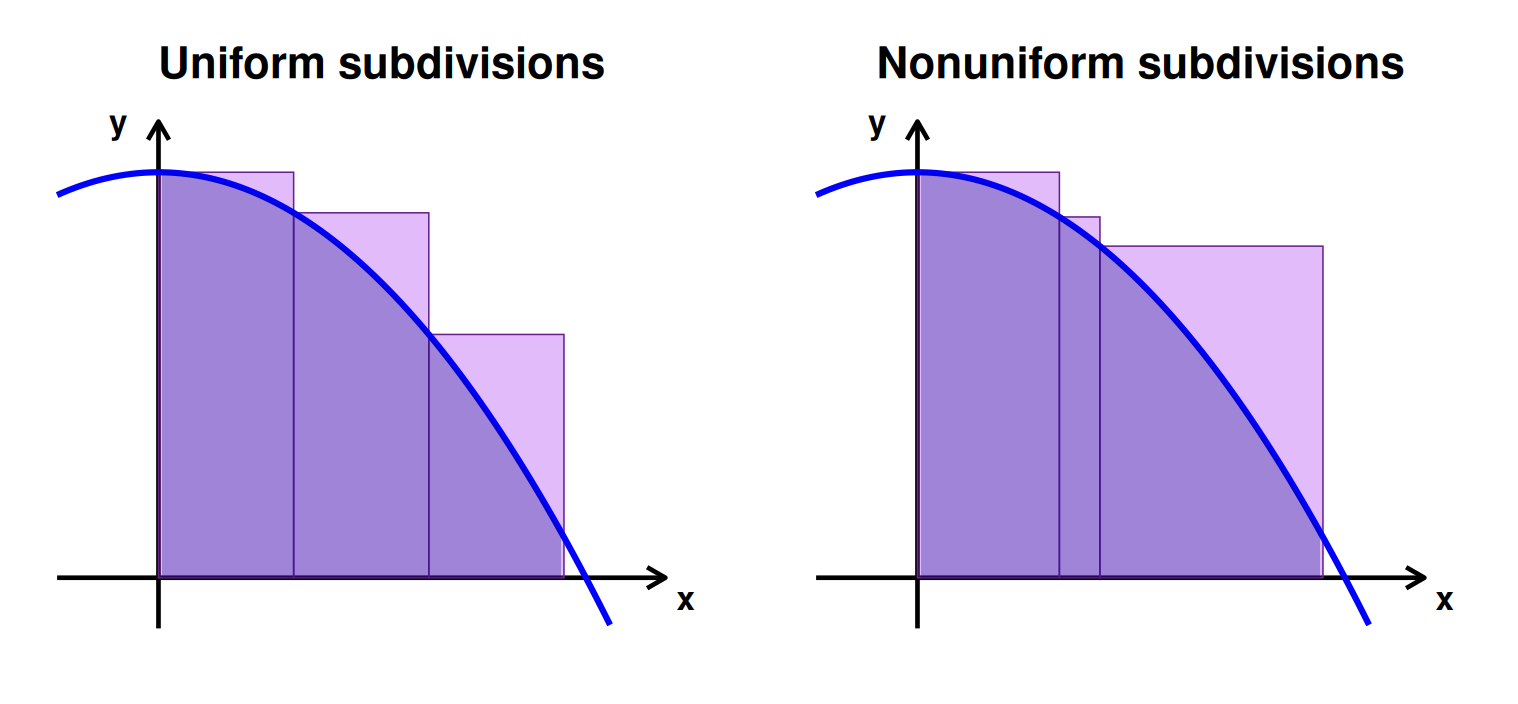
\includegraphics[width=\textwidth]{types-of-partitions.png} 
    \caption{Comparison of uniform and non-uniform partitions of an interval (generated using R).}
    \label{fig:discontinuity}
\end{figure}

\begin{tcolorbox}[breakable]
    A partition of $[a, b]$ divides it into $n$ subintervals:
    \[
    P = \{ a = x_0 < x_1 < x_2 < \dots < x_n = b \}
    \]
    Each subinterval has width:
    \[
    \Delta x_i = x_i - x_{i-1}.
    \]
    \begin{itemize}
        \item \textbf{Uniform Partition:} All subintervals have the same width:
        \[
        \Delta x_i = \Delta x = \frac{b-a}{n}, \quad \forall i.
        \]
        \item \textbf{Non-Uniform Partition:}  Subintervals have different widths, and \( \Delta x_i \) varies for each \( i \).
    \end{itemize}
\end{tcolorbox}


% TYPES OF RIEMANN SUMS

\subsection{Types of Riemann Sums}

\begin{tcolorbox}[breakable]
    The type of Riemann sum depends on how the sample points $x_i^*$ are chosen within each subinterval $[x_{i-1}, x_i]$.
    \begin{enumerate}
        \item \textbf{Arbitrary-Point Rule:} $x_i^* \in [x_{i-1}, x_i] \rightarrow$ \textbf{General Riemann Sum}
        \[
        S_n = \sum_{i=1}^{n} f(x_i^*) \Delta x_i, \quad \Delta x_i = x_i - x_{i-1}.
        \]
        \textbf{Uniform Partition:} If all subintervals have equal width $\Delta x = \frac{b-a}{n}$, then \\ $x_i^* \in [x_{i-1}, x_i] = [a + (i - 1) \Delta x, a + i \Delta x]$ or $x_i^* = a + (i - 1 + c) \Delta x$, where $c \in [0,1]$ determines its position within the subinterval:
        \[
        S_n = \sum_{i=1}^{n} f(a + (i - 1 + c) \Delta x) \Delta x = \sum_{i=1}^{n} f(a + (i - 1 + c) \frac{(b - a)}{n}) \frac{b - a}{n}.
        \]
        $\bullet$ Uses arbitrary sample points $x_i^*$.
    
        \item \textbf{Left Rule:} $x_i^* = x_{i-1}\rightarrow$ \textbf{Left Riemann Sum}
        \[
        S_{\text{left}} = \sum_{i=1}^n f(x_{i-1}) \Delta x_i.
        \]
        \textbf{Uniform Partition:} $c = 0$
        \[
        S_{\text{left}} = \sum_{i=1}^n f(a + (i - 1) \Delta x) \Delta x.
        \]
        $\bullet$ Underestimates for increasing functions, overestimates for decreasing functions.
        
        \item \textbf{Right Rule:} $x_i^* = x_i\rightarrow$ \textbf{Right Riemann Sum}
        \[
        S_{\text{right}} = \sum_{i=1}^n f(x_i) \Delta x_i    
        \]
        \textbf{Uniform Partition:} $c = 1$
        \[
        S_{\text{right}} = \sum_{i=1}^n f(a + i \Delta x) \Delta x.
        \]
        $\bullet$ Overestimates for increasing functions, underestimates for decreasing functions.
        
        \item \textbf{Midpoint Rule:} $x_i^* = \frac{x_{i-1} + x_i}{2} \rightarrow$ \textbf{Midpoint Riemann Sum}
        \[
        S_{\text{mid}} = \sum_{i=1}^n f\left( \frac{x_{i-1} + x_i}{2} \right) \Delta x_i.
        \]
        \textbf{Uniform Partition:} $c = \frac{1}{2}$
        \[
        S_{\text{mid}} = \sum_{i=1}^n f(a + (i - \frac{1}{2}) \Delta x) \Delta x.
        \]
        $\bullet$ Tends to give better approximations than left or right sums.
        
        \item \textbf{Upper Rule:} $x_i^* = \arg\sup\limits_{x \in [x_{i-1}, x_i]} f(x) \rightarrow$ \textbf{Upper Riemann Sum} (or \textbf{Upper Darboux Sum})
        \[
        S_{\text{upper}} = \sum_{i=1}^n \sup\limits_{x \in [x_{i-1}, x_i]} f(x) \Delta x_i.
        \]
        $\bullet$ Always \textbf{overestimates} the integral.

        \pagebreak
        
        \item \textbf{Lower Rule:} $x_i^* = \arg\inf\limits_{x \in [x_{i-1}, x_i]} f(x) \rightarrow$ \textbf{Lower Riemann Sum} (or \textbf{Lower Darboux Sum})
        \[
        S_{\text{lower}} = \sum_{i=1}^n \inf\limits_{x \in [x_{i-1}, x_i]} f(x) \Delta x_i.
        \]
        $\bullet$ Always \textbf{underestimates} the integral.
    \end{enumerate}
\end{tcolorbox}


% DEFINITE INTEGRAL


\subsection{Definite Integral}

\begin{tcolorbox}
    The \textbf{definite integral} of a function $f(x)$ over the interval $[a,b]$ is defined as the limit of a Riemann sum:
    \[
    \int_{a}^{b} f(x) \, dx = \lim_{n \to \infty} \sum_{i=1}^n f(x_i^*) \Delta x_i
    \]
    where:
    \begin{itemize}
        \item $[a,b]$ is divided into $n$ subintervals.
        \item $\Delta x_i = x_i - x_{i-1}$ is the width of the $i$-th subinterval.
        \item $x_i^*$ is any sample point in the $i$-th subinterval.
    \end{itemize}
\end{tcolorbox}
\pagebreak


% PROPERTIES OF DEFINITE INTEGRALS


\subsection{Properties of Definite Integrals}

\begin{tcolorbox}[breakable]
    Let $f(x)$ and $g(x)$ be integrable functions on $[a,b]$ and $c$ be a constant. Then:
    \[
    \begin{aligned}
        &\text{(1)} \quad \int_{a}^{b}c \, dx = c(b-a). \\[8pt]
        &\text{(2)} \quad \int_{a}^{a}f(x) \, dx = 0. \\[8pt]
        &\text{(3)} \quad \int_{b}^{a}f(x) \, dx = -\int_{a}^{b}f(x) \, dx. \\[8pt]
        &\text{(4)} \quad \int_{a}^{b}cf(x) \, dx = c \int_{a}^{b}f(x) \, dx. \\[8pt]
        &\text{(5)} \quad \int_{a}^{b}\left[f(x) \pm g(x)\right] \, dx = \int_{a}^{b}f(x) \, dx \pm \int_{a}^{b}g(x) \, dx. \\[8pt]
        &\text{(6)} \quad \int_{a}^{b}f(x) \, dx = \int_{a}^{c}f(x) \, dx + \int_{c}^{b}f(x) \, dx. \\[8pt]
        &\text{(7)} \quad \int_{a}^{b}f(x) \, dx \leq \int_{a}^{b}g(x) \, dx \quad \text{ if } f(x) \leq g(x) \text{ on } [a,b]. \\[8pt]
        &\text{(8)} \quad \left| \int_{a}^{b}f(x) \, dx \right| \leq \int_{a}^{b} \left|f(x)\right| \, dx. \\[8pt]
        &\text{(9)} \quad m(b-a) \leq \int_{a}^{b}f(x) \, dx \leq M(b-a) \quad \text{ if } m \leq f(x) \leq M \text{ on } [a,b]. \\[8pt]
    \end{aligned}
    \]
\end{tcolorbox}


% NET AND TOTAL AREA


\subsection{Net and Total Area}

\begin{tcolorbox}
    Let $f(x)$ be integrable on $[a,b]$. Define:
    \begin{itemize}
        \item $A_1$ = area of region where $f(x) > 0$ (area above $x$-axis).
        \item $A_2$ = area of region where $f(x) < 0$ (area below $x$-axis).
    \end{itemize}
    Then:
    \begin{itemize}
        \item \textbf{Net Area:}
        \[
        \int_{a}^{b} f(x) \, dx = A_1 - A_2.
        \]
        \item \textbf{Total Area:}
        \[
        \int_{a}^{b} \left| f(x) \right| \, dx = A_1 + A_2.
        \]
    \end{itemize}
\end{tcolorbox}


% MEAN VALUE THEOREM FOR INTEGRALS


\subsection{Mean Value Theorem for Integrals}

\begin{tcolorbox}
    Let $f$ be continuous on [a,b]. Then:
    \[
    \exists c \in (a,b) \text{ such that } \frac{1}{b - a} \int_{a}^{b} f(x) \, dx = f(c)
    \]
    The expression on the left is the \textbf{average value} of the function $f(x)$ on the interval $[a, b]$.
\end{tcolorbox}


% FUNDAMENTAL THEOREM OF CALCULUS. PART 1


\subsection{Fundamental Theorem of Calculus. Part 1}

\begin{tcolorbox}
    Let $f$ be a continuous on $[a, b]$. Define the function
    \[
    F(x) = \int_{a}^{x} f(t) \, dt.
    \]
    Then:
    \[
    F'(x) = \frac{d}{dx} \left[ \int_{a}^{x} f(t) \, dt \right] = f(x), \quad \forall x \in (a,b).
    \]
\end{tcolorbox}


% FUNDAMENTAL THEOREM OF CALCULUS. PART 2


\subsection{Fundamental Theorem of Calculus. Part 2}

\begin{tcolorbox}
    If $f$ is continuous on $[a,b]$ and $F'(x) = f(x)$, then
    \[
    \int_{a}^{b} f(x) \, dx = F(b) - F(a) =  F(x) \bigg]_{a}^{b} = F(x) \bigg|_{a}^{b}.
    \]
\end{tcolorbox}


% TABLE OF INDEFINITE INTEGRALS


\subsection{Table of Indefinite Integrals}

\begin{tcolorbox}[breakable]
    \keepXColumns
    \begin{tabularx}{\textwidth}{X|X}
        $\int a \, dx = ax + C$ &  
        $\int \log_a x \, dx = \frac{x}{\ln{a}} (\ln{x} - 1) + C$ \\[12pt] 

        $\int x^n \, dx = \frac{x^{n+1}}{n+1} + C,\quad n \neq -1$ &
        $\int (ax+b)^n \, dx = \frac{(ax+b)^{n+1}}{a(n+1)} + C$ \\[12pt]
        
        $\int x^{-1} \, dx = \int \frac{1}{x} \, dx = \ln{|x|} + C$ &
        $\int \frac{c}{ax+b} \, dx = \frac{c}{a} \ln{|ax+b|} + C$ \\[12pt] 
        
        $\int e^{ax} \, dx = \frac{1}{a} e^{ax} + C$ &
        $\int a^x \, dx = \frac{a^x}{\ln{a}} + C,\quad a > 0,\; a \neq 1$ \\[12pt]
              
        $\int \sin{x} \, dx = - \cos{x} + C$ &
        $\int \tan{x} \, dx = \ln{|\sec{x}|} = - \ln{|\cos{x}|} + C$ \\[12pt]
              
        $\int \cos{x} \, dx = \sin{x} + C$ &
        $\int \cot{x} \, dx = -\ln{|\csc{x}|} = \ln{|\sin{x}|} + C$ \\[12pt]
        
        $\int \sec{x} \, dx = \ln{|\sec{x} + \tan{x}|} + C$ &
        $\int \sec^2{x} \, dx = \tan{x} + C$ \\[12pt]
        
        $\int \csc{x} \, dx = \ln{|\csc{x} - \cot{x}|} + C$ &
        $\int \csc^2{x} \, dx = -\cot{x} + C$ \\[12pt]
        
        $\int \sec{x} \tan{x} \, dx = \sec{x} + C$ &
        $\int \frac{1}{\sqrt{1-x^2}} \, dx = \arcsin{x} + C$ \\[12pt]
        
        $\int \csc{x} \cot{x} \, dx = -\csc{x} + C$ &
        $\int \frac{1}{1+x^2} \, dx = \arctan{x} + C$ \\[12pt]
    \end{tabularx}
\end{tcolorbox}


% --------------------------------------------------


\section{Sequences and Series}


% DEFINITION OF A SEQUENCE


\subsection{Definition of a Sequence}

\begin{tcolorbox}
    A sequence is a function $a: \mathbb{N} \rightarrow \mathbb{R}$ that assigns to each $n \in N$ a real number $a_n$.
    \[
    \{a_n\} = \{a_n\}_{n=1}^{\infty} = (a_n) = \{a_1, a_2, a_3, \dots, a_n, \dots\}
    \]
\end{tcolorbox}


% MONOTONIC SEQUENCE


\subsection{Monotonic Sequence}

\begin{tcolorbox}
    A sequence $\{a_n\}$ is \textbf{monotonic} if it is either monotonically increasing or monotonically decreasing.
    \begin{itemize}
        \item \textbf{Increasing:}
        \[ a_n \leq a_{n+1}, \quad \forall n \in \mathbb{N} \text{ (weakly increasing)}. \]
        \[ a_n < a_{n+1}, \quad \forall n \in \mathbb{N} \text{ (strictly increasing)}. \]
        \item \textbf{Decreasing:}
        \[ a_n \geq a_{n+1}, \quad \forall n \in \mathbb{N} \text{ (weakly decreasing)}. \]
        \[ a_n > a_{n+1}, \quad \forall n \in \mathbb{N} \text{ (strictly decreasing)}. \]
    \end{itemize}
\end{tcolorbox}


% BOUNDED SEQUENCE


\subsection{Bounded Sequence}

\begin{tcolorbox}
    A sequence $\{a_n\}$ is \textbf{bounded} if and only if:
    \[
    \exists M > 0 \text{ such that } |a_n| \leq M, \quad \forall n \in \mathbb{N}.
    \]
    or
    \[ 
    \exists M_1, M_2 \in \mathbb{R} \text{ such that } M_1 \leq a_n \leq M_2, \quad \forall n \in \mathbb{N}.
    \]
    Equivalently, $\{a_n\}$ is \textbf{bounded} if it is both \textbf{bounded above} and \textbf{bounded below}:
    \begin{itemize}
        \item \textbf{Bounded above:} $\exists M_2 \in \mathbb{R}$ such that $a_n \leq M_2, \quad \forall n \in \mathbb{N}$.
        \item \textbf{Bounded below:} $\exists M_1 \in \mathbb{R}$ such that $a_n \geq M_1, \quad \forall n \in \mathbb{N}$.
    \end{itemize}
    \[
    \text{A sequence is bounded} \iff \text{It is both bounded above and bounded below}
    \]
\end{tcolorbox}


% LIMIT OF A SEQUENCE


\subsection{Limit of a Sequence}

\begin{tcolorbox}
    A sequence $\{a_n\}$ has a limit $L \in \mathbb{R}$ if:
    \[
    \lim_{n \to \infty} a_n = L \quad \text{if} \quad \forall \varepsilon>0, \, \, \exists N \in \mathbb{N} \text{ such that } |a_n - L| < \varepsilon, \, \forall n \geq N.
    \]
    If such an $L$ exists, the sequence is \textbf{convergent}; otherwise, it is \textbf{divergent}.
\end{tcolorbox}


% LIMIT OF A SEQUENCE DEFINED BY A FUNCTION


\subsection{Limit of a Sequence Defined by a Function}

\begin{tcolorbox}
    Let $f: \mathbb{R} \to \mathbb{R}$ be a function and $\{a_n\}$ be defined by $a_n = f(n)$. Then:
    \[
    \lim_{x \to \infty} f(x) = L \implies \lim_{n \to \infty} a_n = L.
    \]
\end{tcolorbox}


% SQUEEZE THEOREM FOR SEQUENCES


\subsection{Squeeze Theorem for Sequences}

\begin{tcolorbox}
    If $a_n \leq b_n \leq c_n$ for all $n \geq N$, then:
    \[
    \lim_{n \to \infty} a_n = \lim_{n \to \infty} c_n = L \implies \lim_{n \to \infty} b_n = L.
    \]
\end{tcolorbox}


% LIMIT OF ABSOLUTE VALUE OF A SEQUENCE


\subsection{Limit of Absolute Value of a Sequence}

\begin{tcolorbox}
    \[
    \lim_{n \to \infty} | a_n | = 0 \implies \lim_{n \to \infty} a_n = 0.
    \]
\end{tcolorbox}


% MONOTONE CONVERGENCE THEOREM


\subsection{Monotone Convergence Theorem}

\begin{tcolorbox}
    Every bounded and monotonic sequence is convergent.
    \[
    \begin{aligned}
        &\text{(1)} \quad \text{Monotonic } \land \text{ Bounded} 
        \implies \text{Convergent}. \\[8pt]
        &\text{(2)} \quad \text{Monotonically Increasing } \land \text{ Bounded Above} 
        \implies \text{Convergent}. \\[8pt]
        &\text{(3)} \quad \text{Monotonically Decreasing } \land \text{ Bounded Below} 
        \implies \text{Convergent}. \\[8pt]
    \end{aligned}
    \]
\end{tcolorbox}


% SERIES


\subsection{Series}

\begin{tcolorbox}
    An \textbf{infinite series} is the sum of the terms of a sequence $\{a_n\}$:
    \[
    \sum_{n=1}^{\infty} a_n = a_1 + a_2 + a_3 + \dots
    \]
    The \textbf{$\boldsymbol{n}^\text{th}$ partial sum} of series:
    \[
    S_n = \sum_{k=1}^{n} a_k.
    \]
\end{tcolorbox}


% CONVERGENCE AND DIVERGENCE OF SERIES


\subsection{Convergence and Divergence of Series}

\begin{tcolorbox}
    A infinite series $\textstyle \sum a_n$ \textbf{converges} if the sequence of partial sums $\{ S_n \}$ has a finite limit:
    \[
    \sum_{k=1}^{\infty} a_k = \lim_{n \to \infty} \sum_{k=1}^{n} a_k \quad \text{or} \quad \lim_{n \to \infty} S_n = S.
    \]
    Otherwise, the series \textbf{diverges}.
\end{tcolorbox}


% TYPES OF SERIES


\subsection{Types of Series}

\begin{tcolorbox}
    \begin{multicols}{3}
        \begin{itemize}
          \item Arithmetic Series
          \item Geometric Series
          \item Arithmetico-Geometric Series
          \item Harmonic Series
          \item p-Series
          \item Telescoping Series
          \item Alternating Series
          \item Power Series
          \item Taylor Series
          \item Maclaurin Series
          \item Taylor Series
          \item Laurent Series
          \item Fourier Series
          \item Binomial Series
          \item Mercator Series
        \end{itemize}
    \end{multicols}
\end{tcolorbox}


% PROPERTIES OF SERIES


\subsection{Properties of Series}

\begin{tcolorbox}
    Let $\textstyle \sum a_n$ and $\textstyle \sum b_n$ be series, and let $c, d$ be a constant. Then:
    \[
    \begin{aligned}
        &\text{(1)} \quad \sum_{k=a}^b c = c(b - a + 1). \\[8pt]  
        &\text{(2)} \quad \sum_{n=k}^{\infty} \pm c = \pm \infty, \quad c > 0. \\[8pt]
        &\text{(3)} \quad \sum_{n=k}^{m} (ca_n \pm db_n) = c \sum_{n=k}^{m} a_n \pm d \sum_{n=k}^{m} b_n. \\[8pt]
        &\text{(4)} \quad \sum_{n=k}^{m} a_n = \sum_{n=k}^{p} a_n + \sum_{n=p+1}^{m} a_n. \\[8pt]
        &\text{(5)} \quad \sum_{n=k}^{m} a_n = \sum_{n=0}^{m-k} a_{m-n}. \\[8pt]
        &\text{(6)} \quad \sum_{n=k}^{m} a_n = \sum_{j=k-h}^{m-h} a_{j+h}. \\[8pt]
        &\text{(7)} \quad \sum_{k=1}^n k = \sum_{k=0}^{n-1} (k + 1). \\[8pt]
    \end{aligned}
    \]
\end{tcolorbox}


% GEOMETRIC SERIES


\subsection{Geometric Series}

\begin{tcolorbox}
    \[
    \text{Geometric} \implies \sum_{n=0}^{\infty} ar^n = a + ar + ar^2 + ar^3 + \dots
    \]
    \begin{itemize}
        \item \textbf{Partial Sum:}
        \[ S_n = \sum_{k=0}^{n-1} ar^k = a \frac{1-r^n}{1-r}, \quad r\neq1. \]
        \item \textbf{Convergence:}
        \[ |r| < 1 \implies \sum_{n=0}^{\infty} ar^n = \frac{a}{1-r}. \]
        \item \textbf{Divergence:}
        \[ |r| \geq 1 \implies \text{Series diverges.} \]
    \end{itemize}
\end{tcolorbox}


% TELESCOPING SERIES


\subsection{Telescoping Series}

\begin{tcolorbox}
    \[
    \text{Telescoping} \implies \sum_{n=1}^{\infty} (a_n - a_{n+1}) = (a_1 - a_2) + (a_2 - a_3) + (a_3 - a_4) + \dots
    \]
    \begin{itemize}
        \item \textbf{Partial Sum:}
        \[ S_n = \sum_{k=1}^{n} (a_k - a_{k+1}) = (a_1 - a_2) + (a_2 - a_3) + \dots + (a_n - a_{n+1}) = a_1 - a_{n+1}. \]
        \item \textbf{Convergence:}
        \[ \lim_{n \to \infty} a_{n+1} = L \implies \sum_{n=1}^{\infty} (a_n - a_{n+1}) = a_1-L. \]
        \item \textbf{Divergence:}
        \[ \lim_{n \to \infty} a_{n+1} \text{ does not exist} \implies \text{Series diverges.} \]
    \end{itemize}
\end{tcolorbox}


% HARMONIC SERIES


\subsection{Harmonic Series}

\begin{tcolorbox}
    \[
    \text{Harmonic} \implies \sum_{n=1}^{\infty} \frac{1}{n} = 1 + \frac{1}{2} + \frac{1}{3} + \frac{1}{4} + \dots
    \]
    \begin{itemize}
        \item \textbf{Partial Sum and Approximation:}
        \[ H_n = \sum_{k=1}^{n} \frac{1}{k} = 1 + \frac{1}{2} + \dots + \frac{1}{n} \approx \ln(n) + \gamma \]
        where $\gamma \approx 0.57721$ is the Euler-Mascheroni constant.
        \item \textbf{Divergence:}
        \[ \sum_{n=1}^{\infty} \frac{1}{n} = \infty \text{ even though } \lim_{n\to\infty} \frac{1}{n} = 0. \]
    \end{itemize}
\end{tcolorbox}


% LIMIT OF TERMS IN A CONVERGENT SERIES


\subsection{Limit of Terms in a Convergent Series}

\begin{tcolorbox}
    Let $\{a_n\}$ be a sequence and $\textstyle \sum a_n$ be its series. Then:
    \[
    \sum a_n \text{ convergent} \implies \lim_{n \to \infty} a_n = 0.
    \]
    Note: The converse is false. ($\textstyle \lim_{n \to \infty} a_n = 0 \centernot\implies \sum a_n \text{ convergent}$)
\end{tcolorbox}


% LIST OF CONVERGENCE TESTS


\subsection{List of Convergence Tests}

\begin{tcolorbox}
    \begin{itemize}
        \item \textbf{Tests for Positive Series:}
        \begin{multicols}{2}
            \begin{itemize}[label=$\circ$]
                \item Direct Comparison Test
                \item Limit Comparison Test
                \item Integral Test % (Maclaurin-Cauchy Test)
                \item p-Series Test
            \end{itemize}
        \end{multicols}
        \item \textbf{Tests for Alternating Series:}
        \begin{multicols}{2}
            \begin{itemize}[label=$\circ$]
                \item Alternating Series Test % (Leibniz Criterion)
                \item Dirichlet’s Test
            \end{itemize}
        \end{multicols}
        \item \textbf{General Tests:}
        \begin{multicols}{2}
            \begin{itemize}[label=$\circ$]
                \item Divergence Test % (nth-Term Test)
                \item Ratio Test % (d'Alembert's Criterion)
                \item Root Test % (Cauchy's Criterion)
                \item Absolute Convergence Test
            \end{itemize}
        \end{multicols}
        \item \textbf{Advanced or Specialized Tests:}
        \begin{multicols}{2}
            \begin{itemize}[label=$\circ$]
                \item Cauchy Condensation Test
                \item Abel's Test 
                \item Raabe's Test
                \item Kummer's Test
                \item Gauss's Test
                \item Bertrand's Test
            \end{itemize}
        \end{multicols}
    \end{itemize}
\end{tcolorbox}


% DIVERGENCE TEST


\subsection{Divergence Test (\emph{n}th-Term Test)}

\begin{tcolorbox}
    \[
    \lim_{n \to \infty} a_n \neq 0 \; \lor \; \lim_{n \to \infty} a_n \text{ does not exist} \implies \sum a_n \text{ diverges}.
    \]
\end{tcolorbox}


% DIRECT COMPARISON TEST


\subsection{Direct Comparison Test}

\begin{tcolorbox}
    If $0 \leq a_n \leq b_n$ for all $n \geq N$:
    \[
    \begin{aligned}
        &\bullet \quad \sum b_n \text{ converges} \implies \sum a_n \text{ converges}. \\[8pt]  
        &\bullet \quad \sum a_n \text{ diverges} \implies \sum b_n \text{ diverges}.
    \end{aligned}
    \]
\end{tcolorbox}


% LIMIT COMPARISON TEST


\subsection{Limit Comparison Test}

\begin{tcolorbox}
    Let $\textstyle \sum a_n$ and $\textstyle \sum b_n$ be series with $a_n > 0,\, b_n > 0$ for all $n \geq N$. Define the limit:
    \[
    L = \lim_{n \to \infty} \frac{a_n}{b_n}.
    \]
    \[
    \begin{aligned}
        &\bullet \quad 0 < L < \infty \implies \sum a_n \text{ and } \sum b_n \text{ both converge or both diverge}. \\[8pt]  
        &\bullet \quad L = 0 \; \land \; \sum b_n \text{ converges} \implies \sum a_n \text{ converges}. \\[8pt]
        &\bullet \quad L = \infty \; \land \; \sum b_n \text{ diverges} \implies \sum a_n \text{ diverges}.
    \end{aligned}
    \]
    Note: The order of division does not matter.
\end{tcolorbox}


% INTEGRAL TEST


\subsection{Integral Test (Maclaurin-Cauchy Test)}

\begin{tcolorbox}
    For a series $\textstyle \sum a_n$ where $a_n = f(n)$, if $f(x)$ is a positive, continuous, and decreasing function for all $x \geq N$, then:
    \[
    \begin{aligned}
        &\bullet \quad \sum_{n=N}^{\infty} a_n \text{ converges} \iff \int_{N}^{\infty} f(x) \, dx \text{ converges}. \\[8pt]  
        &\bullet \quad \sum_{n=N}^{\infty} a_n \text{ diverges} \iff \int_{N}^{\infty} f(x) \, dx \text{ diverges}.
    \end{aligned}
    \]
\end{tcolorbox}


% P-SERIES TEST

\subsection{\emph{p}-Series Test}

\begin{tcolorbox}
    For the \emph{p}-series $\sum_{n=1}^{\infty} \frac{1}{n^p}$, where $p \in \mathbb{R}$:
    \[
    \begin{aligned}
        &\bullet \quad p > 1 \iff \text{Series converges}. \\[8pt]  
        &\bullet \quad p \leq 1 \iff  \text{Series diverges}.
    \end{aligned}
    \]
\end{tcolorbox}


% INTEGRAL REMAINDER ESTIMATE


\subsection{Integral Remainder Estimate}

\begin{tcolorbox}
    For a convergent series $\textstyle \sum_{n=1}^{\infty} a_n$ with $a_n = f(n)$, where $f(x)$ is positive, continuous, and decreasing for all $x \geq N$, if the remainder $R_n = S - S_n$ then
    \[
    \int_{n+1}^{\infty} f(x) \, dx \leq R_n \leq \int_n^{\infty} f(x) \, dx
    \]
    \[
    S_n + \int_{n+1}^{\infty} f(x) \, dx  \leq S \leq S_n + \int_n^{\infty} f(x) \, dx
    \]
\end{tcolorbox}


% ALTERNATING SERIES TEST


\subsection{Alternating Series Test (Leibniz Criterion)}

\begin{tcolorbox}
    For an alternating series $\sum_{n=1}^{\infty} (-1)^{n-1} a_n$, where $a_n > 0$, the series converges if:
    \begin{itemize}
        \item $\lim_{n \to \infty} a_n = 0$. (terms approach zero)
        \item $a_{n+1} \leq a_n$ for all $n \geq N$. (monotonically decreasing)
    \end{itemize}
\end{tcolorbox}


% ALTERNATING SERIES ESTIMATION THEOREM


\subsection{Alternating Series Estimation Theorem}

\begin{tcolorbox}
    For an alternating series approximated by its \emph{n}th partial sum, the absolute error (or remainder) is less than or equal to the absolute value of the next term in the series.
    \[
    |R_n| = |S - S_n| \; \leq \; a_{n+1} = |S_{n+1} - S_n|.
    \]
\end{tcolorbox}


% RATIO TEST


\subsection{Ratio Test (d'Alembert's Criterion)}

\begin{tcolorbox}
    Let $\textstyle \sum a_n$ be an infinite series with $a_n \neq 0$. Define the limit:
    \[
    L = \lim_{n \to \infty} \left| \frac{a_{n+1}}{a_n} \right|.
    \]
    \[
    \begin{aligned}
        &\bullet \quad L < 1 \implies \sum a_n \text{ converges absolutely}. \\[8pt]  
        &\bullet \quad L > 1 \; \lor \; L = \infty \implies \sum a_n \text{ diverges}. \\[8pt]
        &\bullet \quad L = 1 \implies \text{Test is inconclusive}.
    \end{aligned}
    \]
\end{tcolorbox}


% ROOT TEST


\subsection{Root Test (Cauchy's Criterion)}

\begin{tcolorbox}
    Let $\textstyle \sum a_n$ be an infinite series. Define the limit:
    \[
    L = \lim_{n \to \infty} \sqrt[n]{ \left| a_n \right| } = \lim_{n \to \infty} { \left| a_n \right| } ^ {1/n}.
    \]
    \[
    \begin{aligned}
        &\bullet \quad L < 1 \implies \sum a_n \text{ converges absolutely}. \\[8pt]  
        &\bullet \quad L > 1 \; \lor \; L = \infty \implies \sum a_n \text{ diverges}. \\[8pt]
        &\bullet \quad L = 1 \implies \text{Test is inconclusive}.
    \end{aligned}
    \]
\end{tcolorbox}


% ABSOLUTE CONVERGENCE TEST


\subsection{Absolute Convergence Test}

\begin{tcolorbox}
    \begin{itemize}
        \item \textbf{Absolute Convergence:}
        \[
        \sum \left| a_n \right| \text{ converges} \implies \sum a_n \text{ converges absolutely}.
        \]
        \item \textbf{Conditional Convergence:}
        \[
        \left(\sum a_n \text{ converges} \right) \land \left(\sum \left| a_n \right| \text{ diverges} \right) \implies \sum a_n \text{ converges conditionally}.
        \]        
    \end{itemize}
    Note: All rearrangements of absolutely convergent series converge to the same sum.
\end{tcolorbox}


% RIEMANN SERIES THEOREM


\subsection{Riemann Series Theorem}

\begin{tcolorbox}
    Conditionally convergent series $\textstyle \sum_{n=1}^{\infty} a_n$ can be rearranged to:
    \begin{itemize}
        \item Converge to any real number: $\; \textstyle \forall M \in \mathbb{R}, \, \exists \sigma$ such that $\sum_{n=1}^{\infty} a_{\sigma (n)} = M$.
        \item Diverge to $\pm \infty$: $\;  \textstyle \exists \sigma$ such that $\sum_{n=1}^{\infty} a_{\sigma (n)} = \pm \infty$.
        \item Fail to approach any limit: $\;  \exists \sigma$ such that $\lim_{N \to \infty} \sum_{n=1}^N a_{\sigma (n)}$ does not exist.
    \end{itemize}
\end{tcolorbox}


% POWER SERIES


\subsection{Power Series}

\begin{tcolorbox}
    A power series centered at $c$ is an infinite series of the form
    \[
    \sum_{n=0}^{\infty} a_n (x-c)^n = a_0 + a_1 (x - c) + a_2 (x - c)^2 + \dots
    \]
    where $\{a_n\}$ is a sequence of coefficients, $x$ is a variable, and $c$ is the center of the series.
\end{tcolorbox}


% RADIUS OF CONVERGENCE


\subsection{Radius of Convergence}

\begin{tcolorbox}
    For a power series $\textstyle \sum_{n=0}^{\infty} a_n (x - c)^n$, the radius of convergence $R$ is a non-negative real number (possibly $0$ or $\infty$) such that:
    \begin{itemize}
        \item If $R = 0$: The series converges only at $x = c$.
        \item If $R = \infty$: The series converges for all values of $x$.
        \item If $0 < R < \infty$:
        \begin{itemize}[label=$\circ$]
            \item The series converges absolutely for $|x - c| < R$.
            \item The series diverges for $|x - c| > R$.
            \item The series may or may not converge at $|x - c| = R$.
        \end{itemize}
    \end{itemize}
    
    \vspace{5pt}
    \hrule
    \vspace{10pt}
    
    \textbf{Ratio Test:}
    \begin{align*}
        \lim_{n \to \infty} \left| \frac{a_{n+1} (x-c)^{n+1}}{a_n (x - c)^n} \right| < 1 &\implies \lim_{n \to \infty} \left| \frac{a_{n+1}}{a_n} \right| \cdot \left| x - c \right| < 1 \\[8pt]
        L \cdot \left| x - c \right| < 1 &\implies \left| x - c \right| < \frac{1}{L} = \frac{1}{\lim_{n \to \infty} \left| \frac{a_{n+1}}{a_n} \right|}
    \end{align*}
    \[ \boxed{R = \frac{1}{L} = \lim_{n \to \infty} \left| \frac{a_n}{a_{n+1}} \right|} \]
    
    \textbf{Root Test:}
    \begin{align*}
        \lim_{n \to \infty} \sqrt[n]{\left| a_n (x - c)^n \right|} < 1 &\implies  \lim_{n \to \infty} \sqrt[n]{\left| a_n \right|} \cdot \left| x - c \right| < 1 \\[8pt]
        L \cdot \left| x - c \right| < 1 &\implies \left| x - c \right| < \frac{1}{L} = \frac{1}{\lim_{n \to \infty} \sqrt[n]{ \left| a_n \right|}}
    \end{align*}
    \[ \boxed{R = \frac{1}{L} = \frac{1}{\lim_{n \to \infty} \sqrt[n]{|a_n|}}} \]
\end{tcolorbox}


% INTERVAL OF CONVERGENCE


\subsection{Interval of Convergence}

\begin{tcolorbox}
    The interval of convergence of a power series $\textstyle \sum_{n=0}^{\infty} a_n (x - c)^n$ is the set of values of $x$ for which the series converges absolutely.
    \begin{itemize}
        \item If $R = 0$, the interval is $\{ c \}$.
        \item If $R = \infty$, the interval is $(-\infty, +\infty)$.
        \item If $0 < R < \infty$, the interval is one of the following depending on the convergence at the endpoints:
        \begin{multicols}{4}
            \begin{itemize}[label=$\circ$]
                \item $(c - R, c + R)$
                \item $[c - R, c + R)$
                \item $(c - R, c + R]$
                \item $[c - R, c + R]$
            \end{itemize}
        \end{multicols}
    \end{itemize}
\end{tcolorbox}


% DIFFERENTIATION AND INTEGRATION OF POWER SERIES


\subsection{Differentiation and Integration of Power Series}

\begin{tcolorbox}
    For a power series centered at $c$
    \[ f(x) = \sum_{n=0}^{\infty} a_n (x - c)^n = a_0 + a_1 (x - c) + a_2 (x - c)^2 + a_3 (x - c)^3 + \dots \] 
    with radius of convergence $R$: \\[10pt]
    $\bullet$ \textbf{Differentiation:}
    \[
    f'(x) = \frac{d}{dx} \left[ \sum_{n=0}^{\infty} a_n (x - c)^n  \right] = 0 + a_1 + 2 a_2 (x - c) + 3 a_3 (x - c)^2 + \dots
    \]
    \[ \boxed{f'(x) = \sum_{n=1}^{\infty} na_n(x-c)^{n-1}} \]
    
    $\bullet$ \textbf{Integration:}
    \[
    \int f(x) \, dx = \int \sum_{n=0}^{\infty} a_n (x - c)^n \, dx = C + a_0 (x - c) + \frac{a_1}{2} (x - c)^2 + \frac{a_2}{3} (x - c)^3 + \dots 
    \]
    \[ \boxed{\int f(x) \, dx = C + \sum_{n=0}^{\infty} \frac{a_n}{n+1} (x-c)^{n+1}} \]
    Note: Both operations preserve the radius of convergence $R$, however, convergence at the endpoints $x = c \pm R$ may change and must be checked separately.
\end{tcolorbox}


% TAYLOR SERIES


\subsection{Taylor Series}

\begin{tcolorbox}
    Let $f$ be infinitely differentiable at a point $a$. The Taylor Series of $f$ centered at $a$ is the infinite series
    \begin{align*}
        f(x) &= \sum_{n=0}^{\infty} \frac{f^{(n)}(a)}{n!} (x-a)^n \\
        &= f(a) + f'(a) (x-a) + \frac{f''(a)}{2!} (x-a)^2 + \frac{f'''(a)}{3!} (x-a)^3 + \dots
    \end{align*}
    If there exists an interval where $\textstyle f(x) = \sum_{n=0}^{\infty} \frac{f^{(n)}(a)}{n!} (x-a)^n$, then $f$ is analytic at $a$. Note that analyticity implies infinite differentiability, but the converse is false.
\end{tcolorbox}


% TAYLOR POLYNOMIAL


\subsection{Taylor Polynomial}

\begin{tcolorbox}
    The \emph{n}th degree Taylor polynomial of a function $f(x)$ at point $a$ is the finite sum:
    \begin{align*}
        P_n(x) &= \sum_{k=0}^n \frac{f^{(k)}(a)}{k!} (x-a)^k \\
        &= f(a) + f'(a) (x-a) + \frac{f''(a)}{2!} (x-a)^2 + \dots + \frac{f^{(n)}(a)}{n!} (x-a)^n.
    \end{align*}
\end{tcolorbox}


% TAYLOR'S THEOREM


\subsection{Taylor's Theorem}

\begin{tcolorbox}
    Let $f$ be a function that is $n+1$ times differentiable on an open interval $I$ containing a point $a$. Then for any $x \in I$, there exists a point $\xi$ between $a$ and $x$ such that:
    \begin{align*}
        f(x) &= P_n(x) + R_n(x) \\
        &= \sum_{k=0}^n \frac{f^{(k)}(a)}{k!} (x-a)^k + \frac{f^{(n+1)}(\xi)}{(n+1)!} (x - a)^{n+1}.
    \end{align*}
    Note: $\textstyle R_n(x) =  \frac{f^{(n+1)}(\xi)}{(n+1)!} (x - a)^{n+1}$ is the Lagrange form of the remainder.
\end{tcolorbox}


% TAYLOR'S INEQUALITY


\subsection{Taylor's Inequality}

\begin{tcolorbox}
    Taylor's Inequality provides an upper bound on the error when approximating a function with its Taylor polynomial. Let $f$ be a function that is $n+1$ times differentiable on an open interval containing $a$ and $x$. If there exists a constant $M$ such that $f^{(n+1)} (t) \leq M$ for all $t$ between $a$ and $x$, then:
    \[
    \left| R_n(x) \right| \leq \frac{M}{(n+1)!} \left| x - a \right|^{n+1}.
    \]
\end{tcolorbox}


% BINOMIAL SERIES


\subsection{Binomial Series}

\begin{tcolorbox}
    For any real number $|x|<1$, the binomial series is given by
    \begin{align*}
        (1+x)^\alpha &= \sum_{n=0}^{\infty} \binom{\alpha}{n} x^n \\
        &= 1 + \alpha x + \frac{\alpha(\alpha-1)}{2!}x^2 + \frac{\alpha(\alpha-1)(\alpha-2)}{3!}x^3+\dots
    \end{align*}
    where
    \[
    \binom{\alpha}{n} = \frac{\alpha(\alpha-1)\dots(\alpha-n+1)}{n!}.
    \]
\end{tcolorbox}


% --------------------------------------------------


\section{Multivariable Calculus}


% LIMIT OF A FUNCTION OF TWO VARIABLES


\subsection{Limit of a Function of Two Variables}

\begin{tcolorbox}
    \[
    \lim_{(x,y) \to (a,b)} f(x, y) = L \quad \text{if} \quad \forall \varepsilon > 0, \, \exists \delta > 0 \text{ such that } \forall (x,y) \in D, 
    \]
    \[
    0 < \sqrt{(x-a)^2 +(y-b)^2} < \delta \Rightarrow |f(x, y) - L| < \varepsilon.
    \]
\end{tcolorbox}


% TEST FOR NONEXISTENCE OF A LIMIT


\subsection{Test for Nonexistence of a Limit}

\begin{tcolorbox}
    \begin{multicols}{2}
        \begin{itemize}
            \item \large $\lim_{(x,y) \to (a,b) \text{ along } C_1} f(x,y) = L_1$
            \item \large $\lim_{(x,y) \to (a,b) \text{ along } C_2} f(x,y) = L_2$
        \end{itemize}
    \end{multicols}
    \[
    L_1 \neq L_2 \implies \lim_{(x,y) \to (a,b)} f(x, y) \text{ does not exist.}
    \]
\end{tcolorbox}


% PARTIAL DERIVATIVES


\subsection{Partial Derivatives}

\begin{tcolorbox}
    The \textbf{partial derivative} of a function $f(x,y)$ with respect to $x$ is defined by:
    \[
    f_x(x,y) = \frac{\partial f}{\partial x} = \lim_{h \to 0} \frac{f(x+h,y)-f(x,y)}{h}.
    \]
\end{tcolorbox}


% CLAIRAUT'S THEOREM


\subsection{Clairaut’s Theorem}

\begin{tcolorbox}
    If the mixed partial derivatives exist and are continuous then:
    \[
    \frac{\partial ^2 f}{\partial x \partial y} = \frac{\partial ^2 f}{\partial y \partial x},
    \]
    or equivalently,
    \[
    f_{xy} = f_{yx}.
    \]
\end{tcolorbox}


% EQUATION OF A TANGENT PLANE


\subsection{Equation of a Tangent Plane}

\begin{tcolorbox}
    The \textbf{tangent plane} to the surface $z=f(x,y)$ at the point $(a, b, f(a,b))$ is given by:
    \[
    z = f(a,b) + f_x(a,b)(x-a) + f_y(a,b)(x-y).
    \]
\end{tcolorbox}


% TOTAL DIFFERENTIAL


\subsection{Total Differential}

\begin{tcolorbox}
    \[
    dz = f_x(x,y)dx + f_y(x,y)dy = \frac{\partial z}{\partial x} dx + \frac{\partial z}{\partial y} dy.
    \]
\end{tcolorbox}


% CHAIN RULE FOR A FUNCTION OF TWO VARIABLES


\subsection{Chain Rule For a Function of Two Variables}

\begin{tcolorbox}
    If $z=f(x,y)$ and $x=g(t),y=h(t)$, then:
    \[
    \frac{dz}{dt} = \frac{\partial z}{\partial x} \frac{dx}{dt} + \frac{\partial z}{\partial y} \frac{dy}{dt}.
    \]
\end{tcolorbox}


% IMPLICIT DIFFERENTIATION FOR A FUNCTION OF TWO VARIABLES


\subsection{Implicit Differentiation of a Function of Two Variables}

\begin{tcolorbox}
    If $F(x,y)=0$ where $y$ is implicitly defined as a function of $x$:
    \[
    \frac{dy}{dx} = -\frac{F_x}{F_y} = -\frac{\frac{\partial F}{\partial x}}{\frac{\partial F}{\partial y}}.
    \]    
\end{tcolorbox}


% GRADIENT VECTOR


\subsection{Gradient Vector}

\begin{tcolorbox}
    The \textbf{gradient vector} of a function points in the direction of steepest increase of the function at a given point, with its magnitude representing the rate of that increase. It collects all the partial derivatives of the function into a single vector. \\
    
    The gradient vector of $f(x,y)$ at a point $(x_0,y_0)$ is the vector whose components are the partial derivatives of $f$ at that point.
    \[
    \nabla f(x_0,y_0) = \left( f_x (x_0,y_0),f_y (x_0,y_0) \right)
    \]
    or,
    \[
    \nabla f(x_0,y_0) = \left( \frac{\partial f}{\partial x} (x_0,y_0), \frac{\partial f}{\partial y} (x_0,y_0) \right).
    \]
\end{tcolorbox}


% DIRECTIONAL DERIVATIVE


\subsection{Directional Derivative}

\begin{tcolorbox}
    The \textbf{directional derivative} of a function $f(x,y)$ at a point $(x_0,y_0)$ in the direction of a unit vector $\vec{u}=(u_1, u_2)$, where $ \| \vec{u} \| = 1 $, is the rate of change of $f$ at $(x_0,y_0)$ along the direction $\vec{u}$ and is defined as:
    \[
    D_{\vec{u}} f(x,y) = \lim_{h \to 0} \frac{f(x_0 + hu_1, y_0 + hu_2) - f(x_0,y_0)}{h}
    \]
    If $f(x,y)$ is differentiable at a point $(x_0,y_0)$, the directional derivative of $f$ in the direction of a unit vector $\vec{u}=(u_1,u_2)$ is defined as:
    \[
    D_u f(x_0,y_0) = \frac{\partial f}{\partial x} (x_0,y_0) u_1 + \frac{\partial f}{\partial y} (x_0,y_0) u_2,
    \]
    or equivalently,
    \[
    D_u f(x_0,y_0) = \nabla f(x_0,y_0) \cdot \vec{u}.
    \]
\end{tcolorbox}


% TANGENT PLANE TO A LEVEL SURFACE


\subsection{Tangent Plane to a Level Surface}

\begin{tcolorbox}
    The \textbf{tangent plane} to the level surfact at point $(x_0,y_0,z_0)$ of $F(x,y,z)=c$ is:
    \[
    \nabla F(x_0,y_0,z_0) \cdot (x-x_0,y-y_0,z-z_0)=0,
    \]
    or written out fully,
    \[
    F_x(x_0,y_0,z_0)(x-x_0) + F_y(x_0,y_0,z_0)(y-y_0) + F_z(x_0,y_0,z_0)(z-z_0) = 0.
    \]
\end{tcolorbox}


% MAXIMUM AND MINIMUM VALUES OF A FUNCTION OF TWO VARIABLES


\subsection{Maximum and Minimum Values of a Function of Two Variables}

\begin{tcolorbox}
    \begin{enumerate}
        \item \textbf{Critical Points:} Solve the system of equations
        \[
        \frac{\partial f}{\partial x} (x,y) = 0, \quad \frac{\partial f}{\partial y} (x,y) = 0. 
        \]
        \item \textbf{Second Derivative Test:} Compute the second-order partial derivatives $f_{xx}$, $f_{yy}$, $f_{xy}$ and evaluate the discriminant
        \[
        D(x,y) = f_{xx}(x,y)f_{yy}(x,y) - [f_{xy}(x,y)]^2.
        \]
        \begin{itemize}
            \item If $D>0$ and $f_{xx}(x_0,y_0)>0$: Local minimum.
            \item If $D>0$ and $f_{xx}(x_0,y_0)<0$: Local maximum.
            \item If $D<0$: Saddle point (neither max nor min).
            \item If $D=0$: Inconclusive.
        \end{itemize}
        \item \textbf{Boundary Analysis.}
    \end{enumerate}
\end{tcolorbox}


% PARAMETRIC DERIVATIVE


\subsection{Parametric Derivative}

\begin{tcolorbox}
    If $x=f(t)$ and $y=g(t)$, the derivative of $y$ with respect to $x$ is:
    \[
    \frac{dy}{dx} = \frac{dy/dt}{dx/dt} = \frac{\frac{dy}{dt}}{\frac{dx}{dt}}.
    \]
\end{tcolorbox}


% AREA UNDER A PARAMETRIC CURVE


\subsection{Area Under a Parametric Curve}

\begin{tcolorbox}
    Let a parametric curve be defined by $x=f(t)$ and $y=g(t)$ from $t=a$ to $t=b$. Then, the area is given by:
    \[
    A = \int_{x=f(a)}^{x=f(b)} y \, dx = \int_{t=a}^{t=b} g(t) \cdot f'(t) \, dt.
    \]
\end{tcolorbox}


% ARC LENGTH OF A PARAMETRIC CURVE


\subsection{Arc Length of a Parametric Curve}

\begin{tcolorbox}
    The \textbf{arc length} of a parametric curve defined by $x=f(t)$ and $y=g(t)$ from $t=a$ to $t=b$ is given by:
    \[
    L = \int_{a}^{b} \sqrt{\left( \frac{dx}{dt} \right)^2 + \left( \frac{dy}{dt} \right)^2} \, dt.
    \]
\end{tcolorbox}


% SURFACE AREA OF A SOLID REVOLUTION FOR A PARAMETRIC CURVE


\subsection{Surface Area of a Solid Revolution for a Parametric Curve}

\begin{tcolorbox}
    If the curve, defined by $x=f(t)$ and $y=g(t)$ from $t=a$ to $t=b$, is rotated about the $x$-axis, the surface area $S$ is given by:
    \[
    S = 2\pi \int_{a}^b g(t) \sqrt{\left( \frac{dx}{dt} \right)^2 + \left( \frac{dy}{dt} \right)^2} \, dt.
    \]
\end{tcolorbox}


% POLAR COORDINATES


\subsection{Polar Coordinates}

\begin{tcolorbox}
    \begin{itemize}
        \item \textbf{From Polar to Cartesian:}
        \[
        x = r \cos{(\theta)}, \quad y = r \sin{(\theta)}.
        \]
        \item \textbf{From Cartesian to Polar:}
        \[
        r = \sqrt{x^2 +y^2}, \quad \theta = \arctan{\left(\frac{y}{x} \right)}.
        \]
    \end{itemize}
\end{tcolorbox}


% AREA IN POLAR COORDINATES


\subsection{Area in Polar Coordinates}

\begin{tcolorbox}
    The area $A$ of a region enclosed by a polar curve $r=f(\theta)$ from $\theta=a$ to $\theta=b$ is given by:
    \[
    A=\frac{1}{2} \int_a^b r^2 \, d\theta.
    \]
\end{tcolorbox}


% ARC LENGTH IN POLAR COORDINATES


\subsection{Arc Length in Polar Coordinates}

\begin{tcolorbox}
    The arc length $L$ of a polar curve defined by $r=f(\theta)$ from $\theta=a$ to $\theta=b$ is given by:
    \[
    L = \int_a^b \sqrt{r^2 +\left( \frac{dr}{d\theta} \right)^2} \, d\theta.
    \]
\end{tcolorbox}


% TANGENTS TO POLAR CURVES


\subsection{Tangents to Polar Curves}

\begin{tcolorbox}
    The slope of the tangent line to a polar curve $r=f(\theta)$ at a given point $(r,\theta)$ is given by:
    \[
    \frac{dy}{dx} = \frac{\displaystyle \frac{dr}{d\theta} \sin{(\theta) + r \cos{(\theta)}}}{\displaystyle \frac{dr}{d\theta} \cos{(\theta) - r \sin{(\theta)}}}.
    \]
\end{tcolorbox}


% DOUBLE INTEGRAL


\subsection{Double Integral}

\begin{tcolorbox}
    If $R$ is a bounded region and $f$ is integrable over $R$, then:
    \[
    \iint_R f(x,y) \, dA = \lim_{m,n \to \infty} \sum_{i=1}^m \sum_{j=1}^n f(x_{ij}^*,y_{ij}^*) \Delta A_{ij}.
    \]
\end{tcolorbox}


% ITERATED INTEGRAL


\subsection{Iterated Integral}

\begin{tcolorbox}
    For a function $f(x,y)$ defined over a rectangular region $R=[a,b]\times[c,d]$, the double integral
    \[
    \int_c^d\int_a^b f(x,y) \, dx \, dy.
    \]
\end{tcolorbox}


% AVERAGE VALUE OF A FUNCTION OVER A REGION


\subsection{Average Value of a Function over a Region}

\begin{tcolorbox}
    The average value of $f$ the region $R$ is defined by:
    \[
    f_{avg} = \frac{1}{A(R)} \iint_R f(x,y) \, dA.
    \]
\end{tcolorbox}


% DOUBLE INTEGRAL OVER A GENERAL REGION


\subsection{Double Integral Over a General Region}

\begin{tcolorbox}
    \begin{itemize}
        \item \textbf{Type I Region} (vertical slices):\\
        If $R=\{(x,y) : a \leq x \leq b, g_1(x) \leq y \leq g_2(x)\}$, then:
        \[
        \iint_R f(x,y) \, dA = \int_a^b \int_{g_1(x)}^{g_2(x)} f(x,y) \, dy \, dx.
        \]
        \item \textbf{Type II Region} (horizontal slices):\\
        If $R=\{(x,y) : c \leq y \leq d, h_1(x) \leq x \leq h_2(x)\}$, then:
        \[
        \iint_R f(x,y) \, dA = \int_c^d \int_{h_1(y)}^{h_2(y)} f(x,y) \, dx \, dy.
        \]
    \end{itemize}
\end{tcolorbox}


% DOUBLE INTEGRAL IN POLAR COORDINATES


\subsection{Double Integral in Polar Coordinates}

\begin{tcolorbox}
    The double integral in polar coordinates is given by:
    \[
    \iint_R f(x,y) \, dA = \iint_{R'} f(r \cos{\theta},r \sin{\theta}) r \, dr \, d\theta.
    \]
\end{tcolorbox}


% DOUBLE INTEGRAL IN POLAR COORDINATES OVER A GENERAL REGION


\subsection{Double Integral in Polar Coordinates Over a General Region}

\begin{tcolorbox}
    If $R = \{ (r,\theta) : \alpha \leq \theta \leq \beta, r_1(\theta) \leq r \leq r_2(\theta) \}$, then:
    \[
    \iint_R f(x,y) \, dA = \int_{\alpha}^{\beta} \int_{r_1(\theta)}^{r_2(\theta)} f(r \cos{\theta}, r \sin{\theta}) r \, dr \, d\theta.
    \]
\end{tcolorbox}


\end{document}
